%%
%% This is file `example1empty.tex',
%% generated with the docstrip utility.
%%
%% The original source files were:
%%
%% confproc.dtx  (with options: `example1empty')
%% 
%% This is `example1empty.tex', an example file for the confproc package.
%% Copyright (c) 2011 by Vincent Verfaille <confproc.verfaille@gmail.com>
%% 
%% This file is part of the confproc package.
%% -------------------------------------------
%% 
%% It may be distributed and/or modified under the conditions of the
%% LaTeX Project Public License, either version 1.2 of this license or
%% (at your option) any later version.
%% 
%% The latest version of this license is in
%%   http://www.latex-project.org/lppl.txt
%% and version 1.2 or later is part of all distributions of LaTeX version
%% 1999/12/01 or later.
%% 
%% This file may not be distributed without the original source file
%% `confproc.dtx'.
%% 
%% The list of all files belonging to the confproc package is given in
%% the `readme.txt' file.
%% 
%% For more details, LaTeX the source `confproc.dtx'.
%% 
\documentclass[a4,10pt,oneside,onesidepapers,%
  electronic,% [printed] | electronic
  papers=final,% empty | draft | [final] | countpages
  paperselec=all, %[all] | p_001 | p_fake
  hyperref={bookmarksdepth=1,bookmarksopen,bookmarksopenlevel=0,%
    linkcolor=blue,urlcolor=blue},
colorheaders=black,
colorfooters=black,%
  geometry={text={175truemm,226truemm},% A4 & letter
    inner=0.805in,top=29.15mm,bottom=24.5mm,footskip=9.68mm,voffset=-5mm},letter
]{confprocxmeeting}
%]{confproc}
\usepackage[utf8]{inputenc}
%\usepackage[isolatin]{inputenc}
%\usepackage[T1]{fontenc}
\usepackage{mathptmx}
%\usepackage[landscape]{geometry}
\usepackage{,pdflscape}
\usepackage[super]{nth}
\usepackage{titlesec, blindtext, color}
\definecolor{gray75}{gray}{0.75}
\newcommand{\hsp}{\hspace{20pt}}
\titleformat{\chapter}[hang]{\Huge\bfseries}{\thechapter\hsp\textcolor{gray75}{|}\hsp}{0pt}{\Huge\bfseries}
\renewcommand{\procpdfauthor}{{Editor: AB$^3$C }} 
\renewcommand{\procpdftitle}{Proceedings X-Meeting 2017}
\renewcommand{\procpdfsubject}{Annual Meeting AB$^{3}$ Society} 
\renewcommand{\procchead}{} %
\renewcommand{\proclhead}{{\em \small AB$^{3}$C}}
\pagestyle{fancy}
\fancyhf{}
\cfoot{\thepage}
\author{\procpdfauthor}
\title{\procpdftitle}
\date{October 2017 }
\renewcommand{\PAPERPATH}{papers/}
\makeindex

%%%===========  PROCEEDINGS  ===========
\begin{document}
\frontmatter
\setcounter{page}{1}
\pdfbookmark[0]{Preamble}{preamble}
\pdfbookmark[1]{Cover}{cover}
\maketitle
\newpage

\otherpagestyle
\tableofcontents

%%%==== BEGINNING OF PAPERS ====
\mainmatter
\setcounter{npagespreamble}{\arabic{page}-1}

\chapter{Organizing Committee}

\begin{description}

 \item[AB3C President]: Alan M Durham (USP)

\item[AB3C Vice President]: Ney Lemke (UNESP)

  
\item[AB3C Secretaries]:

\begin{itemize}
 \item Marcelo Brand\~ao (Unicamp) 
 \item  Fabr\'{\i}cio Martins Lopes  (UTFPR)
\end{itemize}

\item[AB3C Financial Department]:

\begin{itemize}
\item Priscila Grynberg (Embrapa)
\item Nicole Scherer (Fiocruz)
\end{itemize}


\item[Poster Session Organizers]:

\begin{itemize}
  \item Robson Francisco de Souza (USP)
\item Nicole Scherer (INCA)
\end{itemize}

 \item[Scientific Comitttee]:

  \begin{itemize}
    \item  Andr\'e Fujita (USP)
    \item  Andr\'e Yoshiaki Kashiwabara (UTFPR)
    \item Arthur Gri\"uuber (USP)
    \item Guilherme Targino Valente (Unesp)
    \item Katlin Brauer Massirer (UNICAMP)
    \item M\'arcio Dom (UFRGS)
    \item Maria Berenice Reynaud Steffens (UFPR)
    \item Robson Francisco de Souza (USP)
  \end{itemize}
\item[Highlight Track Organizer]:
\begin{itemize}
\item Priscila Grynberg (Embrapa)
\item Nicole Scherer (Fiocruz)
\end{itemize} 
\end{description}


\newpage
\chapter{Introduction}
The Brazilian Association of Bioinformatics and Computational Biology (AB3C) is
a scientific society funded in July 12th 2004.
Since its creation, AB3C has been responsible for the annual conference entitled
''X-Meeting'' which is the main Bioinformatics and Computation Biology event in
Brazil. This year its 13th edition occurred in S\~ao Pedro on October
\nth{4}-\nth{6} .

	
Bioinformatics is now a strategic area for Brazil and all Latin America and,
therefore, it is also strategic to the development of Science, Technology and
Economy. The X-Meeting is a Brazilian event with international reach which has
an average of 400 participants. The Conference is an opportunity for students,
researchers and companies to interact and difuse knowledge. The AB3C has been a
pioneer society in the field of Bioinformatics in Brazil and we have a history
of ten past very productive meetings.

\begin{figure}[h]
    \begin{center}
  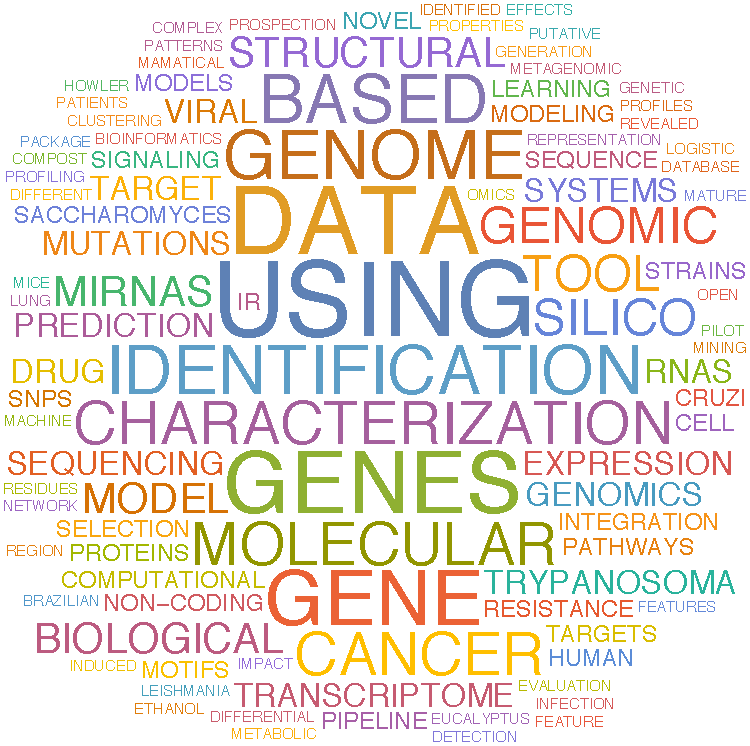
\includegraphics[scale=0.7]{wordcloud}
\end{center}
\caption{Word Cloud for the words used on the Conference Papers Titles}
\end{figure}


\begin{landscape}
\begin{figure}[h]
    \begin{center}
  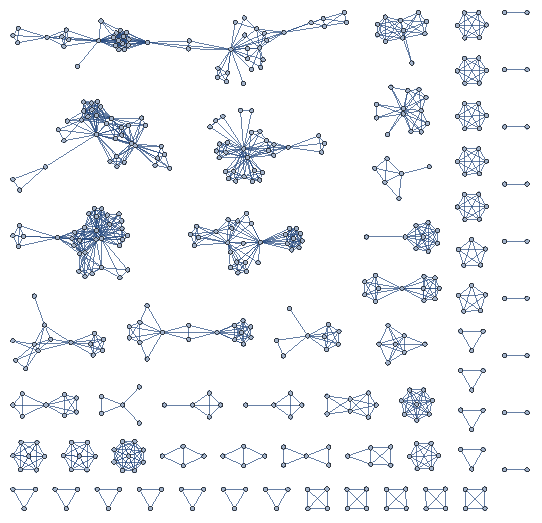
\includegraphics[scale=1.5,angle=0]{grafo}
\end{center}
\caption{Graph representing the network of collaborations of the X-meeting 2016. An interactive 
version of this graph can be seen at \url{https://neylemke.github.io/assets/grafo.html}}
\end{figure}
\end{landscape}

%\chapter{Abstracts}

\procday{Poster Session}
\chapter{Genes and Genomics}
\procpaper[switch=45,
    title={Preliminary association of putative GBS-based SNPs with brown rust resistance phenotypes in a sugarcane map population using GWAS and machine learning methods}, 
    author={Alexandre Hild Aono, James Shiniti Nagai, Estela Araujo Costa, Hugo Rody Vianna Silva, Fernanda Raquel Camilo dos Santos, Luciana Rossini Pinto, Anete Pereira de Souza, Reginaldo Massanobu Kuroshu}, 
    index={{\index{Aono,  Alexandre Hild},\index{Nagai,  James Shiniti},\index{Costa,  Estela Araujo},\index{Silva,  Hugo Rody Vianna},\index{Santos,  Fernanda Raquel Camilo dos},\index{Pinto,  Luciana Rossini},\index{Souza,  Anete Pereira de},\index{Kuroshu,  Reginaldo Massanobu}}}]
    {art61622} 

 \procpaper[switch=45,
    title={Identification and analysis of thermophilic protein sequences in compost sequencing data}, 
    author={Amanda Rodrigues, Aline Maria da Silva, João Carlos Setubal}, 
    index={{\index{Rodrigues,  Amanda},\index{Silva,  Aline Maria da},\index{Setubal,  João Carlos}}}]
    {art61670} 

 \procpaper[switch=45,
    title={CNV calling and its characterization in the Brazilian population}, 
    author={Ana Claudia Martins Ciconelle, Júlia Maria Pavan Soler}, 
    index={{\index{Ciconelle,  Ana Claudia Martins},\index{Soler,  Júlia Maria Pavan}}}]
    {art61260} 

 \procpaper[switch=45,
    title={Copy number variations of genomic and transcriptomic motifs of Mucin and MASP superfamilies in different Trypanosoma cruzi strains}, 
    author={Anderson Coqueiro dos Santos, Gabriela Flavia Rodrigues Luiz, Najib M. El-Sayed, Santuza Maria Ribeiro Teixeira, João Luís Reis Cunha, Daniella Bartholomeu}, 
    index={{\index{Santos,  Anderson Coqueiro dos},\index{Luiz,  Gabriela Flavia Rodrigues},\index{El-Sayed,  Najib M.},\index{Teixeira,  Santuza Maria Ribeiro},\index{Cunha,  João Luís Reis},\index{Bartholomeu,  Daniella}}}]
    {art61684} 

 \procpaper[switch=45,
    title={The Pan-Genome of Treponema pallidum Reveals Differences in Genome Plasticity between the subspecies}, 
    author={Arun Kumar Jaiswal, Sandeep Tiwari, Syed Babar Jamal Bacha, Vasco a de C Azevedo, Siomar de Castro Soares}, 
    index={{\index{Jaiswal,  Arun Kumar},\index{Tiwari,  Sandeep},\index{Bacha,  Syed Babar Jamal},\index{Azevedo,  Vasco a de C},\index{Soares,  Siomar de Castro}}}]
    {art61617} 

 \procpaper[switch=45,
    title={Homology detection using multilayer maximum clustering coefficient}, 
    author={Caio Rafael do Nascimento Santiago, Luciano Antonio Digiampietri}, 
    index={{\index{Santiago,  Caio Rafael do Nascimento},\index{Digiampietri,  Luciano Antonio}}}]
    {art60677} 

 \procpaper[switch=45,
    title={New approach for genomic comparison of invasive and non-invasive strains of Streptococcus pyogenes}, 
    author={Suzane de Andrade Barboza, Caio Rafael do Nascimento Santiago, Luciano Antonio Digiampietri}, 
    index={{\index{Barboza,  Suzane de Andrade},\index{Santiago,  Caio Rafael do Nascimento},\index{Digiampietri,  Luciano Antonio}}}]
    {art61030} 

 \procpaper[switch=45,
    title={Development of an integrated genetic map for a full-sib progeny from crossing between Eucalyptus grandis and Eucalyptus urophylla}, 
    author={Cristiane Hayumi Taniguti, Izabel Christina Gava de Souza, Shinitiro Oda, Leandro de Siqueira, Rodrigo Neves Graça, Thiago Romanos Benatti, José Luiz Stape, Antonio Augusto Franco Garcia}, 
    index={{\index{Taniguti,  Cristiane Hayumi},\index{Souza,  Izabel Christina Gava de},\index{Oda,  Shinitiro},\index{Siqueira,  Leandro de},\index{Graça,  Rodrigo Neves},\index{Benatti,  Thiago Romanos},\index{Stape,  José Luiz},\index{Garcia,  Antonio Augusto Franco}}}]
    {art61556} 

 \procpaper[switch=45,
    title={Gene expression biclustering with FIrefly Algorithm}, 
    author={Denilson Oliveira Melo, Paulo Eduardo Ambrósio}, 
    index={{\index{Melo,  Denilson Oliveira},\index{Ambrósio,  Paulo Eduardo}}}]
    {art56287} 

 \procpaper[switch=45,
    title={MARVEL: A pipeline for recovery and analysis of viral genomes from metagenomic shotgun sequencing data}, 
    author={Deyvid Amgarten, Aline Maria da Silva, João Carlos Setubal}, 
    index={{\index{Amgarten,  Deyvid},\index{Silva,  Aline Maria da},\index{Setubal,  João Carlos}}}]
    {art61242} 

 \procpaper[switch=45,
    title={Biovar equi versus ovis: What genetically differentiate them?}, 
    author={Doglas Parise, Mariana Teixeira Dornelles Parise, Marcus Vinicius Canário Viana, Elma Lima Leite, Anne Cybelle Pinto Gomide, Vasco Ariston de Carvalho Azevedo}, 
    index={{\index{Parise,  Doglas},\index{Parise,  Mariana Teixeira Dornelles},\index{Viana,  Marcus Vinicius Canário},\index{Leite,  Elma Lima},\index{Gomide,  Anne Cybelle Pinto},\index{Azevedo,  Vasco Ariston de Carvalho}}}]
    {art58959} 

 \procpaper[switch=45,
    title={Ploidy level analysis of functional SNPs from GBS data in a sugarcane map population}, 
    author={Estela Araujo Costa, Alexandre Hild Aono, Hugo Rody Vianna Silva, James Shiniti Nagai, Anete Pereira de Souza, Reginaldo Massanobu Kuroshu}, 
    index={{\index{Costa,  Estela Araujo},\index{Aono,  Alexandre Hild},\index{Silva,  Hugo Rody Vianna},\index{Nagai,  James Shiniti},\index{Souza,  Anete Pereira de},\index{Kuroshu,  Reginaldo Massanobu}}}]
    {art61578} 

 \procpaper[switch=45,
    title={Lower proportion than expected for transversions and higher for transitions in synonymous SNPs evaluated in dbSNP}, 
    author={Fernanda Stussi, Tetsu Sakamoto, José Miguel Ortega}, 
    index={{\index{Stussi,  Fernanda},\index{Sakamoto,  Tetsu},\index{Ortega,  José Miguel}}}]
    {art61710} 

 \procpaper[switch=45,
    title={Comparative genomics of six Pseudomonas phages isolated from composting}, 
    author={Fernando Pacheco Nobre Rossi, Deyvid Amgarten, João Carlos Setubal, Aline Maria da Silva}, 
    index={{\index{Rossi,  Fernando Pacheco Nobre},\index{Amgarten,  Deyvid},\index{Setubal,  João Carlos},\index{Silva,  Aline Maria da}}}]
    {art61472} 

 \procpaper[switch=45,
    title={Analysis of genomic islands of virulence and pathogenicity in Xanthomonas campestris}, 
    author={Juan Carlos Ariute, João Pacifico Bezerra Neto, Ana Maria Benko-Iseppon, Flavia Figueira Aburjaile}, 
    index={{\index{Ariute,  Juan Carlos},\index{Neto,  João Pacifico Bezerra},\index{Benko-Iseppon,  Ana Maria},\index{Aburjaile,  Flavia Figueira}}}]
    {art58374} 

 \procpaper[switch=45,
    title={Comparative genomics of Xanthomonas spp. focusing on CAZymes associated with host-pathogen specificity}, 
    author={Gabriela Persinoti, Mario Tyago Murakami}, 
    index={{\index{Persinoti,  Gabriela},\index{Murakami,  Mario Tyago}}}]
    {art61087} 

 \procpaper[switch=45,
    title={GBKFinisher: A tool for GenBank files refinement}, 
    author={Gustavo Santos de Oliveira, Doglas Parise, Mariana Teixeira Dornelles Parise, Anne Cybelle Pinto Gomide, Vasco Ariston de Carvalho Azevedo}, 
    index={{\index{Oliveira,  Gustavo Santos de},\index{Parise,  Doglas},\index{Parise,  Mariana Teixeira Dornelles},\index{Gomide,  Anne Cybelle Pinto},\index{Azevedo,  Vasco Ariston de Carvalho}}}]
    {art61503} 

 \procpaper[switch=45,
    title={Analysis of metagenomic data from howler monkeys feces}, 
    author={Italo Sudre Pereira, Raquel Riyuzo de Almeida Franco, Layla Martins, Julio Oliveira, João Carlos Setubal, Aline Maria da Silva}, 
    index={{\index{Pereira,  Italo Sudre},\index{Franco,  Raquel Riyuzo de Almeida},\index{Martins,  Layla},\index{Oliveira,  Julio},\index{Setubal,  João Carlos},\index{Silva,  Aline Maria da}}}]
    {art61597} 

 \procpaper[switch=45,
    title={Identification of genes under positive selection in Corynebacterium pseudotuberculosis}, 
    author={Marcus Vinicius Canário Viana, Henrique Figueiredo, Felipe Luiz Pereira, Fernanda Alves Dorella, Anne Cybelle Pinto Gomide, Alice Rebecca Wattam, Vasco a de C Azevedo}, 
    index={{\index{Viana,  Marcus Vinicius Canário},\index{Figueiredo,  Henrique},\index{Pereira,  Felipe Luiz},\index{Dorella,  Fernanda Alves},\index{Gomide,  Anne Cybelle Pinto},\index{Wattam,  Alice Rebecca},\index{Azevedo,  Vasco a de C}}}]
    {art61667} 

 \procpaper[switch=45,
    title={Identification of motifs in the promoter region of genes related to the ABA-dependent pathway in sugarcane}, 
    author={Mauro de Medeiros Oliveira, Alan Durham, Glaucia Souza Mendes}, 
    index={{\index{Oliveira,  Mauro de Medeiros},\index{Durham,  Alan},\index{Mendes,  Glaucia Souza}}}]
    {art61634} 

 \procpaper[switch=45,
    title={CAATINGA SOIL MICROBIOME: an ecological and biotechnological overview revealed by omics approaches}, 
    author={Melline Fontes Noronha, Gileno Vieira Lacerda Junior, Renan Abib Pastore, Valéria Maia de Oliveira}, 
    index={{\index{Noronha,  Melline Fontes},\index{Junior,  Gileno Vieira Lacerda},\index{Pastore,  Renan Abib},\index{Oliveira,  Valéria Maia de}}}]
    {art61447} 

 \procpaper[switch=45,
    title={Bioinformatic Analysis of Ubiquitin-Specific Protease Genes in Genome of Phaseoulus vulgaris L.}, 
    author={Monize Angela de Andrade, Daniel Alexandre Azevedo, Laurence Rodrigues do Amaral, Felipe Teles Barbosa, Enyara Rezende Morais, Matheus de Souza Gomes}, 
    index={{\index{Andrade,  Monize Angela de},\index{Azevedo,  Daniel Alexandre},\index{Amaral,  Laurence Rodrigues do},\index{Barbosa,  Felipe Teles},\index{Morais,  Enyara Rezende},\index{Gomes,  Matheus de Souza}}}]
    {art53697} 

 \procpaper[switch=45,
    title={Gene Assembly, Prediction and Phylogenomic Analysis of Erianthus arundinaceus, a crop for biomass production}, 
    author={Nicholas Vinicius Silva, Luciana Souto Mofatto, Juliana José, Gonçalo Amarante Guimarães Pereira, Marcelo Falsarella Carazzolle}, 
    index={{\index{Silva,  Nicholas Vinicius},\index{Mofatto,  Luciana Souto},\index{José,  Juliana},\index{Pereira,  Gonçalo Amarante Guimarães},\index{Carazzolle,  Marcelo Falsarella}}}]
    {art61587} 

 \procpaper[switch=45,
    title={Genomic analysis of Corynebacterium pseudotuberculosis strain 262}, 
    author={Raquel Enma Hurtado Castillo, Marcus Vinicius Canário Viana, Anne Cybelle Pinto Gomide, Vasco A. de C. Azevedo, Rommel Thiago Jucá Ramos, Artur Silva}, 
    index={{\index{Castillo,  Raquel Enma Hurtado},\index{Viana,  Marcus Vinicius Canário},\index{Gomide,  Anne Cybelle Pinto},\index{Azevedo,  Vasco A. de C.},\index{Ramos,  Rommel Thiago Jucá},\index{Silva,  Artur}}}]
    {art61644} 

 \procpaper[switch=45,
    title={16S rRNA GENE-BASED PROFILING OF HOWLER MONKEY FECAL MICROBIOTA}, 
    author={Raquel Riyuzo de Almeida Franco, Júlio César O. Franco, João Carlos Setubal, Aline Maria da Silva}, 
    index={{\index{Franco,  Raquel Riyuzo de Almeida},\index{Franco,  Júlio César O.},\index{Setubal,  João Carlos},\index{Silva,  Aline Maria da}}}]
    {art61610} 

 \procpaper[switch=45,
    title={A graph-based approach to explore local structures in genome graphs aiming the identification of genetic variants}, 
    author={Rodrigo Theodoro Rocha, Georgios Joannis Pappas Junior}, 
    index={{\index{Rocha,  Rodrigo Theodoro},\index{Junior,  Georgios Joannis Pappas}}}]
    {art61646} 

 \procpaper[switch=45,
    title={An NGS approach to analysing HMF resistance in Saccharomyces cerevisiae}, 
    author={Lucas Miranda, Sheila Tiemi Nagamatsu, Fellipe Melo, Bruna Tatsue, Gonçalo Amarante Guimarães Pereira, Gleidson Silva Teixeira, Marcelo Falsarella Carazzolle}, 
    index={{\index{Miranda,  Lucas},\index{Nagamatsu,  Sheila Tiemi},\index{Melo,  Fellipe},\index{Tatsue,  Bruna},\index{Pereira,  Gonçalo Amarante Guimarães},\index{Teixeira,  Gleidson Silva},\index{Carazzolle,  Marcelo Falsarella}}}]
    {art61668} 

 \procpaper[switch=45,
    title={Respiratory nitrate reductase metabolic pathway in Corynebacterium pseudotuberculosis biovar Equi}, 
    author={Sintia Almeida, Vasco a de C Azevedo}, 
    index={{\index{Almeida,  Sintia},\index{Azevedo,  Vasco a de C}}}]
    {art61666} 

 \procpaper[switch=45,
    title={Microbial diversity of inocula and mature compost from thermophilic composting operation at the São Paulo Zoo}, 
    author={Suzana Eiko Sato Guima, Laís Uchôa Rabelo Mendes, Roberta Verciano Pereira, Layla Martins, Aline Maria da Silva, João Carlos Setubal}, 
    index={{\index{Guima,  Suzana Eiko Sato},\index{Mendes,  Laís Uchôa Rabelo},\index{Pereira,  Roberta Verciano},\index{Martins,  Layla},\index{Silva,  Aline Maria da},\index{Setubal,  João Carlos}}}]
    {art61549} 

 \procpaper[switch=45,
    title={Oncogenic Fusion Gene CD74-NRG1 Confers Cancer Stem Cell-like Properties in Lung Cancer through a IGF2 Autocrine/Paracrine Circuit.}, 
    author={Takahiko Murayama, Tatsunori Nishimura, Kana Tominaga, Asuka Nakata, Noriko Gotoh}, 
    index={{\index{Murayama,  Takahiko},\index{Nishimura,  Tatsunori},\index{Tominaga,  Kana},\index{Nakata,  Asuka},\index{Gotoh,  Noriko}}}]
    {art56205} 

 \procpaper[switch=45,
    title={A predictive alignment-free model based on a new logistic regression-based method for feature selection in complete and partial sequences of Senecavirus A}, 
    author={Tatiana Flávia Pinheiro de Oliveira, Marcos Augusto dos Santos, Marcelo Fernandes Camargos, Antônio Augusto Fonseca Júnior, Aristóteles Góes-Neto, Edel Figueiredo Barbosa Stancioli}, 
    index={{\index{Oliveira,  Tatiana Flávia Pinheiro de},\index{Santos,  Marcos Augusto dos},\index{Camargos,  Marcelo Fernandes},\index{Júnior,  Antônio Augusto Fonseca},\index{Góes-Neto,  Aristóteles},\index{Stancioli,  Edel Figueiredo Barbosa}}}]
    {art61466} 

 \procpaper[switch=45,
    title={Acylsugar pathway in Solanum lycopersicum and Solanum pennellii}, 
    author={Thaís Cunha de Sousa Cardoso, Carolina Milagres Caneschi, Fernandes-Brum C. N., Matheus Martins Daude, Gabriel Lasmar dos Reis, Lima A. A, Luiz Antônio Augusto Gomes, Laurence Rodrigues do Amaral, Chalfun-Junior A., Wilson Roberto Maluf, Matheus de Souza Gomes}, 
    index={{\index{Cardoso,  Thaís Cunha de Sousa},\index{Caneschi,  Carolina Milagres},\index{N.,  Fernandes-Brum C.},\index{Daude,  Matheus Martins},\index{Reis,  Gabriel Lasmar dos},\index{A,  Lima A.},\index{Gomes,  Luiz Antônio Augusto},\index{Amaral,  Laurence Rodrigues do},\index{A.,  Chalfun-Junior},\index{Maluf,  Wilson Roberto},\index{Gomes,  Matheus de Souza}}}]
    {art53699} 

 \procpaper[switch=45,
    title={Alignment of the SSR microsatellite markers sequences with the cassava genome (Manihot esculenta)}, 
    author={Vanesca Priscila Camargo Rocha, Daniel Longhi Fernandes Pedro}, 
    index={{\index{Rocha,  Vanesca Priscila Camargo},\index{Pedro,  Daniel Longhi Fernandes}}}]
    {art61456} 

 \procpaper[switch=45,
    title={An analytical pipeline for detection of differential DNA methylation from restriction reduced genomic representation: a pilot study in Eucalyptus.}, 
    author={Wendell Jacinto Pereira, Marilia de Castro Rodrigues Pappas, Dario Grattapaglia, Georgios Joannis Pappas Junior}, 
    index={{\index{Pereira,  Wendell Jacinto},\index{Pappas,  Marilia de Castro Rodrigues},\index{Grattapaglia,  Dario},\index{Junior,  Georgios Joannis Pappas}}}]
    {art61683} 

 \procpaper[switch=45,
    title={Improving variant accuracy with Copy number variant pipeline for target sequencing}, 
    author={George de Vasconcelos Carvalho Neto, Wilder Barbosa Galvao, Marcel Caraciolo, Rodrigo Bertollo, Joao Bosco Oliveira}, 
    index={{\index{Neto,  George de Vasconcelos Carvalho},\index{Galvao,  Wilder Barbosa},\index{Caraciolo,  Marcel},\index{Bertollo,  Rodrigo},\index{Oliveira,  Joao Bosco}}}]
    {art61624} 

 \procpaper[switch=45,
    title={Best Practices for Bioinformatics Pipelines for Molecular-Barcoded Targeted Sequencing}, 
    author={Marcel Caraciolo, Wilder Barbosa Galvao, George de Vasconcelos Carvalho Neto, Rodrigo Bertollo, Joao Bosco Oliveira}, 
    index={{\index{Caraciolo,  Marcel},\index{Galvao,  Wilder Barbosa},\index{Neto,  George de Vasconcelos Carvalho},\index{Bertollo,  Rodrigo},\index{Oliveira,  Joao Bosco}}}]
    {art63645} 

 \chapter{Phylogeny and Evolution}
\procpaper[switch=45,
    title={An Approach to Study Taxonomic Distribution of Genes: Biofilm Production as a Model}, 
    author={Antonio Gilson Gomes Mesquita, Sabrina Sondre de Oliveira Reis Margarido, José Miguel Ortega, Tetsu Sakamoto}, 
    index={{\index{Mesquita,  Antonio Gilson Gomes},\index{Margarido,  Sabrina Sondre de Oliveira Reis},\index{Ortega,  José Miguel},\index{Sakamoto,  Tetsu}}}]
    {art63026} 

 \procpaper[switch=45,
    title={Evolution of Bitopic Signal Transduction Proteins}, 
    author={Aureliano Coelho Proença Guedes, Raphael D. Teixeira, Chuck S. Farah, Robson Francisco de Souza}, 
    index={{\index{Guedes,  Aureliano Coelho Proença},\index{Teixeira,  Raphael D.},\index{Farah,  Chuck S.},\index{Souza,  Robson Francisco de}}}]
    {art61390} 

 \procpaper[switch=45,
    title={Systemic study of the evolution of flowers}, 
    author={Beatriz Moura Kfoury de Castro, Tetsu Sakamoto, Carlos Alberto Xavier Gonçalves, José Miguel Ortega}, 
    index={{\index{Castro,  Beatriz Moura Kfoury de},\index{Sakamoto,  Tetsu},\index{Gonçalves,  Carlos Alberto Xavier},\index{Ortega,  José Miguel}}}]
    {art61467} 

 \procpaper[switch=45,
    title={11.000 Synonymous! But not so much...}, 
    author={Clovis Ferreira dos Reis, Rodrigo Juliani Siqueira Dalmolin, Andre Fonseca, Sandro Jose de Souza}, 
    index={{\index{Reis,  Clovis Ferreira dos},\index{Dalmolin,  Rodrigo Juliani Siqueira},\index{Fonseca,  Andre},\index{Souza,  Sandro Jose de}}}]
    {art56359} 

 \procpaper[switch=45,
    title={THE ORIGIN OF THE GENES OF HUMAN DIGESTIVE SYSTEM SECRETION}, 
    author={Fenícia Brito, Tetsu Sakamoto, José Miguel Ortega}, 
    index={{\index{Brito,  Fenícia},\index{Sakamoto,  Tetsu},\index{Ortega,  José Miguel}}}]
    {art58730} 

 \procpaper[switch=45,
    title={Comparative genomics of bacterial toxins associated with the type IV secretion system}, 
    author={Gianlucca Gonçalves Nicastro, Robson Francisco de Souza}, 
    index={{\index{Nicastro,  Gianlucca Gonçalves},\index{Souza,  Robson Francisco de}}}]
    {art61345} 

 \procpaper[switch=45,
    title={Detection and recontruction of viral haplotypes from APMV-1 samples}, 
    author={Giovanni Marques de Castro, Francisco Pereira Lobo, Helena Lage Ferreira}, 
    index={{\index{Castro,  Giovanni Marques de},\index{Lobo,  Francisco Pereira},\index{Ferreira,  Helena Lage}}}]
    {art61709} 

 \procpaper[switch=45,
    title={Insights about the phylogenomic approaches to Staphylococcus aureus taxa clustering}, 
    author={Guilherme Coppini, Célio Dias Santos Júnior, Flávio Henrique Silva}, 
    index={{\index{Coppini,  Guilherme},\index{Júnior,  Célio Dias Santos},\index{Silva,  Flávio Henrique}}}]
    {art61662} 

 \procpaper[switch=45,
    title={Ancestral reconstruction of transthyretin / 5-hydroxy isourate hydrolase sequences}, 
    author={Lucas Carrijo de Oliveira, Laila Alves Nahum, Lucas Bleicher}, 
    index={{\index{Oliveira,  Lucas Carrijo de},\index{Nahum,  Laila Alves},\index{Bleicher,  Lucas}}}]
    {art61625} 

 \procpaper[switch=45,
    title={Genome assembly completeness and its effect on phylogenetic estimation}, 
    author={Rafael Cabus Gantois, Raquel Enma Hurtado Castillo, Rodrigo Profeta Silveira Santos, Thiago de Jesus Sousa, Marcus Vinicius Canário Viana, Anne Cybelle Pinto Gomide, Artur Silva, Rafael Azevedo Baraúna, Vasco a de C Azevedo}, 
    index={{\index{Gantois,  Rafael Cabus},\index{Castillo,  Raquel Enma Hurtado},\index{Santos,  Rodrigo Profeta Silveira},\index{Sousa,  Thiago de Jesus},\index{Viana,  Marcus Vinicius Canário},\index{Gomide,  Anne Cybelle Pinto},\index{Silva,  Artur},\index{Baraúna,  Rafael Azevedo},\index{Azevedo,  Vasco a de C}}}]
    {art61672} 

 \procpaper[switch=45,
    title={Initial characterization of the blood DNA virome from 1000+ Brazilian elderly individuals}, 
    author={Suzana Andreoli Marques Ezquina, Michel Naslavsky, Maria Rita Passos-Bueno, Mayana Zatz}, 
    index={{\index{Ezquina,  Suzana Andreoli Marques},\index{Naslavsky,  Michel},\index{Passos-Bueno,  Maria Rita},\index{Zatz,  Mayana}}}]
    {art62879} 

 \procpaper[switch=45,
    title={Genome-wide identification of novel miRNAs in cnidarian genomes}, 
    author={Tamires Caixeta Alves, Laurence Rodrigues do Amaral, Matheus de Souza Gomes}, 
    index={{\index{Alves,  Tamires Caixeta},\index{Amaral,  Laurence Rodrigues do},\index{Gomes,  Matheus de Souza}}}]
    {art53706} 

 \chapter{Proteins and Proteomics}
\procpaper[switch=45,
    title={Structural and comparative analyses of fumarate hydratase from three species of Leishmania genus presented in Brazil and their counterpart in human genome.}, 
    author={Aline Beatriz Mello Rodrigues, Ana Carolina Ramos Guimarães}, 
    index={{\index{Rodrigues,  Aline Beatriz Mello},\index{Guimarães,  Ana Carolina Ramos}}}]
    {art61524} 

 \procpaper[switch=45,
    title={Identification of Staphylococcus aureus secretome protein signature using logistic regression to distinguish its role in interaction with the host}, 
    author={Ana Carolina Barbosa Caetano, Sandeep Tiwari, Núbia Seiffert, Vasco a de C Azevedo, Thiago Luiz de Paula Castro}, 
    index={{\index{Caetano,  Ana Carolina Barbosa},\index{Tiwari,  Sandeep},\index{Seiffert,  Núbia},\index{Azevedo,  Vasco a de C},\index{Castro,  Thiago Luiz de Paula}}}]
    {art61570} 

 \procpaper[switch=45,
    title={A Parallel Bioinspired approach to the Protein Folding Problem using a coarse-grained model}, 
    author={Andrey Cabral Meira, César Manuel Vargas Benítez}, 
    index={{\index{Meira,  Andrey Cabral},\index{Benítez,  César Manuel Vargas}}}]
    {art61606} 

 \procpaper[switch=45,
    title={Integrated model of the mRNA translation and the amino acid chain folding within the ribosome tunnel}, 
    author={Bárbara Zanandreiz de Siqueira Mattos, A.P.F. Atman, Anton Semenchenko}, 
    index={{\index{Mattos,  Bárbara Zanandreiz de Siqueira},\index{Atman,  A.P.F.},\index{Semenchenko,  Anton}}}]
    {art57666} 

 \procpaper[switch=45,
    title={In-silico Structural Characterization of Variants Found in PCSK9 gene Identified in Familial Hypercholesterolemic Patients}, 
    author={Bruna Los, Jéssica Bassani Borges, Gisele Medeiros Bastos, André Arpad Faludi, Rosário Dominguez Crespo Hirata, Mario Hiroyuki Hirata}, 
    index={{\index{Los,  Bruna},\index{Borges,  Jéssica Bassani},\index{Bastos,  Gisele Medeiros},\index{Faludi,  André Arpad},\index{Hirata,  Rosário Dominguez Crespo},\index{Hirata,  Mario Hiroyuki}}}]
    {art58471} 

 \procpaper[switch=45,
    title={Aspergillus fumigatus : computational characterization of  UBP14 deubiquitinase}, 
    author={Carlos Bruno de Araujo, Juliana da Silva Viana, Natália Silva da Trindade, Polyane Vieira Macêdo, Matheus de Souza Gomes, Enyara Rezende Morais}, 
    index={{\index{Araujo,  Carlos Bruno de},\index{Viana,  Juliana da Silva},\index{Trindade,  Natália Silva da},\index{Macêdo,  Polyane Vieira},\index{Gomes,  Matheus de Souza},\index{Morais,  Enyara Rezende}}}]
    {art53789} 

 \procpaper[switch=45,
    title={IN SILICO MODELING OF THE C2H2 ZINC-FINGER DOMAIN OF THE GLI3 TRANSCRIPTION FACTOR}, 
    author={Cinthia Caroline Alves, Eduardo Antônio Donadi, Silvana Giuliatti}, 
    index={{\index{Alves,  Cinthia Caroline},\index{Donadi,  Eduardo Antônio},\index{Giuliatti,  Silvana}}}]
    {art58259} 

 \procpaper[switch=45,
    title={A new method based on structural signatures to propose mutations for enzymes ß-glucosidase used in biofuel production}, 
    author={Diego Mariano, Raquel Melo Minardi}, 
    index={{\index{Mariano,  Diego},\index{Minardi,  Raquel Melo}}}]
    {art60933} 

 \procpaper[switch=45,
    title={Evaluation of the molecular impact of an exclusive aminoacid substitution of Saccharomyces cerevisae more tolerant to ethanol strains:  a molecular dynamics approach.}, 
    author={Guilherme Ferreira Luz, Guilherme Targino Valente, Rafael P. Simões}, 
    index={{\index{Luz,  Guilherme Ferreira},\index{Valente,  Guilherme Targino},\index{Simões,  Rafael P.}}}]
    {art62980} 

 \procpaper[switch=45,
    title={Virtual Screening of potential inhibitors for the Alpha-Amylase and Alpha-Glycosidase by shape based model and docking}, 
    author={Heitor Cappato, Nilson Nicolau Junior, Foued Salmen Espindola}, 
    index={{\index{Cappato,  Heitor},\index{Junior,  Nilson Nicolau},\index{Espindola,  Foued Salmen}}}]
    {art53752} 

 \procpaper[switch=45,
    title={Detection and prediction of premature stop codon using mass spectrometry data at the protein level}, 
    author={Karla Cristina Tabosa Machado, Andre Fonseca, Sandro Jose de Souza, Gustavo Antônio de Souza}, 
    index={{\index{Machado,  Karla Cristina Tabosa},\index{Fonseca,  Andre},\index{Souza,  Sandro Jose de},\index{Souza,  Gustavo Antônio de}}}]
    {art61249} 

 \procpaper[switch=45,
    title={Spatial representation of amino acid composition divergence in homologous protein families}, 
    author={Lucas Carrijo de Oliveira, Néli José da Fonseca Júnior, Lucas Bleicher}, 
    index={{\index{Oliveira,  Lucas Carrijo de},\index{Júnior,  Néli José da Fonseca},\index{Bleicher,  Lucas}}}]
    {art61631} 

 \procpaper[switch=45,
    title={Structural features of HIV-1 Integrase mutations in patients and in vitro samples treated with strand transfer Inhibitors}, 
    author={Lucas de Almeida Machado, Ana Carolina Ramos Guimarães}, 
    index={{\index{Machado,  Lucas de Almeida},\index{Guimarães,  Ana Carolina Ramos}}}]
    {art61725} 

 \procpaper[switch=45,
    title={Identification and computational evaluation of possible allosteric and competitive inhibitors of human PEPCK-M: an alternative therapy for lung carcinoma}, 
    author={Luiz Phillippe Ribeiro Baptisa, Vanessa de Vasconcelos Sinatti Castilho, Ana Carolina Ramos Guimarães}, 
    index={{\index{Baptisa,  Luiz Phillippe Ribeiro},\index{Castilho,  Vanessa de Vasconcelos Sinatti},\index{Guimarães,  Ana Carolina Ramos}}}]
    {art61663} 

 \procpaper[switch=45,
    title={In silico improvement of the cyanobacterial lectin microvirin and Mana(1-2)Man interaction}, 
    author={Adonis Lima, Andrei Santos Siqueira, Luiza Möller, Rafael Souza, Alex Ranieri Jerônimo Lima, Ronaldo Correia da Silva, Délia Cristina Figueira Aguiar, João Lídio da Silva Gonçalves Vianez Junior, Evonnildo Costa Gonçalves}, 
    index={{\index{Lima,  Adonis},\index{Siqueira,  Andrei Santos},\index{Möller,  Luiza},\index{Souza,  Rafael},\index{Lima,  Alex Ranieri Jerônimo},\index{Silva,  Ronaldo Correia da},\index{Aguiar,  Délia Cristina Figueira},\index{Junior,  João Lídio da Silva Gonçalves Vianez},\index{Gonçalves,  Evonnildo Costa}}}]
    {art61728} 

 \procpaper[switch=45,
    title={Low Molecular Weight Phophatases: Coevolved residues and a Mutation Database}, 
    author={Marcelo Querino Lima Afonso, Néli José da Fonseca Júnior, Lucas Bleicher}, 
    index={{\index{Afonso,  Marcelo Querino Lima},\index{Júnior,  Néli José da Fonseca},\index{Bleicher,  Lucas}}}]
    {art61034} 

 \procpaper[switch=45,
    title={Identifying specificity determinant residues through decomposition of protein families affiliation network}, 
    author={Néli José da Fonseca Júnior, Lucas Carrijo de Oliveira, Marcelo Querino Lima Afonso, Lucas Bleicher}, 
    index={{\index{Júnior,  Néli José da Fonseca},\index{Oliveira,  Lucas Carrijo de},\index{Afonso,  Marcelo Querino Lima},\index{Bleicher,  Lucas}}}]
    {art61542} 

 \procpaper[switch=45,
    title={Functional prediction of stress-modulated proteins of Deinococcus radiodurans}, 
    author={Ricardo Valle Ladewig Zappala, Manuela Leal da Silva, Pedro Geraldo Pascutti, Claudia de Alencar Santos Lage}, 
    index={{\index{Zappala,  Ricardo Valle Ladewig},\index{Silva,  Manuela Leal da},\index{Pascutti,  Pedro Geraldo},\index{Lage,  Claudia de Alencar Santos}}}]
    {art58294} 

 \procpaper[switch=45,
    title={Functional analysis of hypothetical proteins unveils putative metabolic pathways, essential genes and Therapeutic drug and vaccine target in Trypanosma cruzi: A Bioinformatics Based Approach}, 
    author={Rodrigo Profeta Silveira Santos, Priya Trivedi, Neha Jain, Sandeep Tiwari, Syed Babar Jamal Bacha, Arun Kumar Jaiswal, Thiago Luiz de Paula Castro, Núbia Seiffert, Siomar de Castro Soares, Artur Silva, Vasco a de C Azevedo}, 
    index={{\index{Santos,  Rodrigo Profeta Silveira},\index{Trivedi,  Priya},\index{Jain,  Neha},\index{Tiwari,  Sandeep},\index{Bacha,  Syed Babar Jamal},\index{Jaiswal,  Arun Kumar},\index{Castro,  Thiago Luiz de Paula},\index{Seiffert,  Núbia},\index{Soares,  Siomar de Castro},\index{Silva,  Artur},\index{Azevedo,  Vasco a de C}}}]
    {art61612} 

 \procpaper[switch=45,
    title={Proteome scale comparative modeling for conserved drug and vaccine targets identification in Salmonella serovers}, 
    author={Syed Babar Jamal Bacha, Jyoti Yadav, Neha Jain, Sandeep Tiwari, Arun Kumar Jaiswal, Thiago Luiz de Paula Castro, Núbia Seiffert, Siomar de Castro Soares, Artur Silva, Vasco a de C Azevedo}, 
    index={{\index{Bacha,  Syed Babar Jamal},\index{Yadav,  Jyoti},\index{Jain,  Neha},\index{Tiwari,  Sandeep},\index{Jaiswal,  Arun Kumar},\index{Castro,  Thiago Luiz de Paula},\index{Seiffert,  Núbia},\index{Soares,  Siomar de Castro},\index{Silva,  Artur},\index{Azevedo,  Vasco a de C}}}]
    {art61604} 

 \procpaper[switch=45,
    title={In silico screening of volatile compounds which can complex with the AeagOBP1 odor-binding protein of Aedes aegypti L.}, 
    author={Tarcisio Silva Melo, Liliane Pereira de Araújo, Rosangela Santos Pereira, Thaís Almeida de Menezes, Wagner Rodrigues de Assis Soares, Bruno Silva Andrade}, 
    index={{\index{Melo,  Tarcisio Silva},\index{Araújo,  Liliane Pereira de},\index{Pereira,  Rosangela Santos},\index{Menezes,  Thaís Almeida de},\index{Soares,  Wagner Rodrigues de Assis},\index{Andrade,  Bruno Silva}}}]
    {art61648} 

 \procpaper[switch=45,
    title={Comparative analysis of the alternative splicing diversity in the human and mouse brain proteomes: preliminary results}, 
    author={Esdras Matheus da Silva, Thais Martins, Raphael Tavares da Silva, Fabio Passetti}, 
    index={{\index{Silva,  Esdras Matheus da},\index{Martins,  Thais},\index{Silva,  Raphael Tavares da},\index{Passetti,  Fabio}}}]
    {art61469} 

 \procpaper[switch=45,
    title={Analysis of splice variants in the proteome of Alzheimer's disease: preliminary results}, 
    author={Thais Martins, Esdras Matheus da Silva, Raphael Tavares da Silva, Fabio Passetti}, 
    index={{\index{Martins,  Thais},\index{Silva,  Esdras Matheus da},\index{Silva,  Raphael Tavares da},\index{Passetti,  Fabio}}}]
    {art61468} 

 \procpaper[switch=45,
    title={Evaluation of differentially expressed proteins during Leishmania major infection in murine macrophages lacking nitric oxide synthase}, 
    author={Victor Hugo Toledo, Djalma de Souza Lima Junior, Lívia Rosa Fernandes, Giuseppe Palmisano, Luiza A. Castro-Jorge, Dario Simões Zamboni}, 
    index={{\index{Toledo,  Victor Hugo},\index{Junior,  Djalma de Souza Lima},\index{Fernandes,  Lívia Rosa},\index{Palmisano,  Giuseppe},\index{Castro-Jorge,  Luiza A.},\index{Zamboni,  Dario Simões}}}]
    {art61593} 

 \procpaper[switch=45,
    title={In silico study of a new Brazilian semi arid compound with possible IKK-ß inhibitory action}, 
    author={Wagner Rodrigues de Assis Soares, Thaís Almeida de Menezes, Bruno Silva Andrade}, 
    index={{\index{Soares,  Wagner Rodrigues de Assis},\index{Menezes,  Thaís Almeida de},\index{Andrade,  Bruno Silva}}}]
    {art61678} 

 \chapter{RNA and Transcriptomics}
\procpaper[switch=45,
    title={IN SILICO IDENTIFICATION, CHARACTERIZATION AND PHYLOGENETIC ANALYSIS OF miRNAs IN WILD PEPPER}, 
    author={Ailton Pereira da Costa Filho, Monize Angela de Andrade, Laurence Rodrigues do Amaral, Matheus de Souza Gomes}, 
    index={{\index{Filho,  Ailton Pereira da Costa},\index{Andrade,  Monize Angela de},\index{Amaral,  Laurence Rodrigues do},\index{Gomes,  Matheus de Souza}}}]
    {art53719} 

 \procpaper[switch=45,
    title={Association of Hfq/LSm protein with insertion sequence-derived RNAs is a prevalent phenomenon in prokaryotes}, 
    author={Alan Péricles Rodrigues Lorenzetti, Lívia S. Zaramela, Joao Paulo Pereira de Almeida, José Vicente Gomes-Filho, Ricardo Zorzetto Nicoliello Vêncio, Tie Koide}, 
    index={{\index{Lorenzetti,  Alan Péricles Rodrigues},\index{Zaramela,  Lívia S.},\index{Almeida,  Joao Paulo Pereira de},\index{Gomes-Filho,  José Vicente},\index{Vêncio,  Ricardo Zorzetto Nicoliello},\index{Koide,  Tie}}}]
    {art61713} 

 \procpaper[switch=45,
    title={Unraveling the lincRNA transcriptome of the mice olfactory system}, 
    author={Antônio Pedro de Castello Branco da Rocha Camargo, Marcelo Falsarella Carazzolle, Fabio Papes}, 
    index={{\index{Camargo,  Antônio Pedro de Castello Branco da Rocha},\index{Carazzolle,  Marcelo Falsarella},\index{Papes,  Fabio}}}]
    {art61498} 

 \procpaper[switch=45,
    title={In silico molecular subtype-specific drug targets prospection by integrating colorectal cancer and tumor-derived cell lines data}, 
    author={Laboratório de Bioinformática E Biologia Computacional, Nicole Scherer, Luís Felipe Ribeiro Pinto, Mariana Boroni}, 
    index={{\index{Computacional,  Laboratório de Bioinformática E Biologia},\index{Scherer,  Nicole},\index{Pinto,  Luís Felipe Ribeiro},\index{Boroni,  Mariana}}}]
    {art61559} 

 \procpaper[switch=45,
    title={PRELIMINARY ANALYSIS OF miRNAs IN THE GENOME OF Citrus sinensis}, 
    author={Douglas Santana, Tamires Caixeta Alves, Laurence Rodrigues do Amaral, Matheus de Souza Gomes}, 
    index={{\index{Santana,  Douglas},\index{Alves,  Tamires Caixeta},\index{Amaral,  Laurence Rodrigues do},\index{Gomes,  Matheus de Souza}}}]
    {art53712} 

 \procpaper[switch=45,
    title={The assessment of the impact of small deletions within human protein domains using transcriptome data: a pilot study in lung cancer}, 
    author={Fernanda Cristina Medeiros de Oliveira, Gabriel Wajnberg, Fabio Passetti}, 
    index={{\index{Oliveira,  Fernanda Cristina Medeiros de},\index{Wajnberg,  Gabriel},\index{Passetti,  Fabio}}}]
    {art61475} 

 \procpaper[switch=45,
    title={CHARACTERIZATION AND INDENTIFICATION OF MATURE miRNAs AND THEIR PRECURSORS IN THE GENOME OF CULTIVATED PEPPER}, 
    author={Fernando Augusto Corrêa Queiroz Cançado, Monize Angela de Andrade, Laurence Rodrigues do Amaral, Matheus de Souza Gomes}, 
    index={{\index{Cançado,  Fernando Augusto Corrêa Queiroz},\index{Andrade,  Monize Angela de},\index{Amaral,  Laurence Rodrigues do},\index{Gomes,  Matheus de Souza}}}]
    {art53742} 

 \procpaper[switch=45,
    title={HIGH-THROUGHPUT SEQUENCING AND DE NOVO ASSEMBLY OF TRANSCRIPTOME OF Vigna unguiculata UPON VIRAL INFECTION}, 
    author={Flavia Figueira Aburjaile, João Pacifico Bezerra Neto, Bruna Piereck Moura, José Ribamar Costa Ferreira-Neto, Ana Maria Benko-Iseppon}, 
    index={{\index{Aburjaile,  Flavia Figueira},\index{Neto,  João Pacifico Bezerra},\index{Moura,  Bruna Piereck},\index{Ferreira-Neto,  José Ribamar Costa},\index{Benko-Iseppon,  Ana Maria}}}]
    {art61695} 

 \procpaper[switch=45,
    title={EVALUATING THE COWPEA DEHYDRATION STRESS TOLERANCE BASED ON INOSITOL AND RAPHINOSIS PATHWAYS}, 
    author={João Pacifico Bezerra Neto, Flavia Figueira Aburjaile, José Ribamar Costa Ferreira-Neto, Ana Maria Benko-Iseppon, MG Santos}, 
    index={{\index{Neto,  João Pacifico Bezerra},\index{Aburjaile,  Flavia Figueira},\index{Ferreira-Neto,  José Ribamar Costa},\index{Benko-Iseppon,  Ana Maria},\index{Santos,  MG}}}]
    {art61691} 

 \procpaper[switch=45,
    title={Comparison of bioinformatics approaches to evaluate altered GO processes in in vivo and in vitro studies of antineoplastics of OPEN TG-GATEs online database}, 
    author={Giordano Bruno, André Luiz Molan, Jose Rybarczyk-Filho}, 
    index={{\index{Bruno,  Giordano},\index{Molan,  André Luiz},\index{Rybarczyk-Filho,  Jose}}}]
    {art61592} 

 \procpaper[switch=45,
    title={Computer-aided protocol to revisit the cDNA library from Lonomia obliqua caterpillar: Identification of structural motifs related to inflammatory processes}, 
    author={Jaqueline Mayara de Araujo, Milton Y. Nishiyama-Jr, Flavio Lichtenstein, Kerly Fernanda Mesquita Pasqualoto, Ana Marisa Chudzinski-Tavassi}, 
    index={{\index{Araujo,  Jaqueline Mayara de},\index{Nishiyama-Jr,  Milton Y.},\index{Lichtenstein,  Flavio},\index{Pasqualoto,  Kerly Fernanda Mesquita},\index{Chudzinski-Tavassi,  Ana Marisa}}}]
    {art61715} 

 \procpaper[switch=45,
    title={Genes and pathways modulated during Guillain-Barré Syndrome}, 
    author={Raulzito Fernandes Moreira, Paulo Ricardo Porfírio do Nascimento, Glória Regina de Góis Monteiro, Mario Emilio Teixeira Dourado Junior, Selma Maria Bezerra Jeronimo, João Paulo Matos Santos Lima}, 
    index={{\index{Moreira,  Raulzito Fernandes},\index{Nascimento,  Paulo Ricardo Porfírio do},\index{Monteiro,  Glória Regina de Góis},\index{Junior,  Mario Emilio Teixeira Dourado},\index{Jeronimo,  Selma Maria Bezerra},\index{Lima,  João Paulo Matos Santos}}}]
    {art61605} 

 \procpaper[switch=45,
    title={Identification and characterization of miRNAs and their targets in cucumber genome}, 
    author={Júlia Silveira Queiroz, Núbia Carolina Pereira Silva, Laurence Rodrigues do Amaral, Matheus de Souza Gomes}, 
    index={{\index{Queiroz,  Júlia Silveira},\index{Silva,  Núbia Carolina Pereira},\index{Amaral,  Laurence Rodrigues do},\index{Gomes,  Matheus de Souza}}}]
    {art53753} 

 \procpaper[switch=45,
    title={High throughput sequencing of small RNAs in Biomphalaria glabrata}, 
    author={Laysa Gomes Portilho, Fábio Ribeiro Queiroz, Wander Jesus Jeremias, Elio Hideo Babá, Roberta Lima Caldeira, Laurence Rodrigues do Amaral, Matheus de Souza Gomes}, 
    index={{\index{Portilho,  Laysa Gomes},\index{Queiroz,  Fábio Ribeiro},\index{Jeremias,  Wander Jesus},\index{Babá,  Elio Hideo},\index{Caldeira,  Roberta Lima},\index{Amaral,  Laurence Rodrigues do},\index{Gomes,  Matheus de Souza}}}]
    {art53695} 

 \procpaper[switch=45,
    title={Comparative analysis of transcriptomes reveals the existence of genes with distinct profiles: overactive genes and gaussian genes}, 
    author={Lissur Azevedo Orsine, Glaura da Conceição Franco, José Miguel Ortega}, 
    index={{\index{Orsine,  Lissur Azevedo},\index{Franco,  Glaura da Conceição},\index{Ortega,  José Miguel}}}]
    {art61615} 

 \procpaper[switch=45,
    title={Combining metagenomics and metatranscriptomics approaches for prospection of CAZymes of the lower termite Coptotermes gestroi}, 
    author={Luciana Souto Mofatto, João Paulo Lourenço Franco Cairo, Melline Fontes Noronha, Ana Maria Costa Leonardo, Fabio Marcio Squina, Gonçalo Amarante Guimarães Pereira, Marcelo Falsarella Carazzolle}, 
    index={{\index{Mofatto,  Luciana Souto},\index{Cairo,  João Paulo Lourenço Franco},\index{Noronha,  Melline Fontes},\index{Leonardo,  Ana Maria Costa},\index{Squina,  Fabio Marcio},\index{Pereira,  Gonçalo Amarante Guimarães},\index{Carazzolle,  Marcelo Falsarella}}}]
    {art61535} 

 \procpaper[switch=45,
    title={Transcriptional evaluation of induced pluripotent cells from patients with Cockayne syndrome after induction of DNA damage triggered by oxidative stress}, 
    author={Maira Rodrigues de Camargo Neves, Livia Luz Souza Nascimento, Alexandre Teixeira Vessoni, Carlos Frederico Martins Menck}, 
    index={{\index{Neves,  Maira Rodrigues de Camargo},\index{Nascimento,  Livia Luz Souza},\index{Vessoni,  Alexandre Teixeira},\index{Menck,  Carlos Frederico Martins}}}]
    {art60122} 

 \procpaper[switch=45,
    title={Finders keepers, nobody weepers! Unraveling novel genes in transcriptomes.}, 
    author={Marina Pupke Marone, Felipe Rodrigues da Silva}, 
    index={{\index{Marone,  Marina Pupke},\index{Silva,  Felipe Rodrigues da}}}]
    {art63597} 

 \procpaper[switch=45,
    title={miRNA, piRNA and snoRNA expression profile analysis in thyroid cancer subtypes}, 
    author={Mayla Abrahim Costa, Natasha Jorge, Fabio Passetti}, 
    index={{\index{Costa,  Mayla Abrahim},\index{Jorge,  Natasha},\index{Passetti,  Fabio}}}]
    {art61481} 

 \procpaper[switch=45,
    title={Occurrence of differential alternative splicing in the transcriptome of mice hearts infected with two strains of Trypanosoma cruzi}, 
    author={Nayara Toledo, Raphael Tavares da Silva, Tiago Bruno Rezende de Castro, Glória Regina Franco, Andrea Mara Macedo, Carlos Renato, Égler Chiari, Neuza Antunes Rodrigues}, 
    index={{\index{Toledo,  Nayara},\index{Silva,  Raphael Tavares da},\index{Castro,  Tiago Bruno Rezende de},\index{Franco,  Glória Regina},\index{Macedo,  Andrea Mara},\index{Renato,  Carlos},\index{Chiari,  Égler},\index{Rodrigues,  Neuza Antunes}}}]
    {art61745} 

 \procpaper[switch=45,
    title={Unraveling the molecular profile of alternative transcripts through analysis of eCLIP and RNA-Seq data}, 
    author={Pedro Rodrigues Sousa da Cruz, Felipe Ciamponi, Katlin Massirer}, 
    index={{\index{Cruz,  Pedro Rodrigues Sousa da},\index{Ciamponi,  Felipe},\index{Massirer,  Katlin}}}]
    {art62074} 

 \procpaper[switch=45,
    title={Comprehensive profiling and characterization of  Arachis stenosperma (peanut) and Meloidogyne arenaria (plant-root nematode) small-RNAs identified during the course of the infection}, 
    author={Priscila Grynberg, Larrisa A. Guimarães, Marcos Mota do Carmo Costa, Roberto Coiti Togawa, Ana Cristina M. Brasileiro, Patricia Messenberg Guimarães}, 
    index={{\index{Grynberg,  Priscila},\index{Guimarães,  Larrisa A.},\index{Costa,  Marcos Mota do Carmo},\index{Togawa,  Roberto Coiti},\index{Brasileiro,  Ana Cristina M.},\index{Guimarães,  Patricia Messenberg}}}]
    {art61409} 

 \procpaper[switch=45,
    title={Metalloproteinases diversity in the venom gland of Peruvian spider Loxosceles laeta revealed by transcriptome analysis}, 
    author={Raissa Medina Santos, Clara Guerra Duarte, Priscilla Alves de Aquino, Anderson Oliveira do Carmo, César Bonilla, Evanguedes Kalapothakis, Carlos Chavez-Olortegui}, 
    index={{\index{Santos,  Raissa Medina},\index{Duarte,  Clara Guerra},\index{Aquino,  Priscilla Alves de},\index{Carmo,  Anderson Oliveira do},\index{Bonilla,  César},\index{Kalapothakis,  Evanguedes},\index{Chavez-Olortegui,  Carlos}}}]
    {art58573} 

 \procpaper[switch=45,
    title={TPP riboswitch analysis using molecular dynamic with different force fields}, 
    author={Rodrigo Bentes Kato, Jadson Claudio Belchior, Debora Antunes}, 
    index={{\index{Kato,  Rodrigo Bentes},\index{Belchior,  Jadson Claudio},\index{Antunes,  Debora}}}]
    {art61324} 

 \procpaper[switch=45,
    title={Annotation of transfer RNAs and microRNAs from Coffea canephora genome}, 
    author={Samara Mireza Correia de Lemos, Alexandre R. Paschoal, Douglas Silva Domingues}, 
    index={{\index{Lemos,  Samara Mireza Correia de},\index{Paschoal,  Alexandre R.},\index{Domingues,  Douglas Silva}}}]
    {art58790} 

 \procpaper[switch=45,
    title={A potential link between tuberculosis and lung cancer through non-coding RNAs}, 
    author={Sandeep Tiwari, Debmalya Barh, Ranjith N. Kumavath, Vasco a de C Azevedo}, 
    index={{\index{Tiwari,  Sandeep},\index{Barh,  Debmalya},\index{Kumavath,  Ranjith N.},\index{Azevedo,  Vasco a de C}}}]
    {art61337} 

 \procpaper[switch=45,
    title={Transcriptome profiles of Resistance Gene Analogs in Saccharum hybrid cultivar RB925345 in response to Sporisorium scitamineum infection}, 
    author={Sintia Almeida, Patricia Dayane Carvalho Schaker, Claudia Barros Monteiro-Vitorello}, 
    index={{\index{Almeida,  Sintia},\index{Schaker,  Patricia Dayane Carvalho},\index{Monteiro-Vitorello,  Claudia Barros}}}]
    {art61561} 

 \procpaper[switch=45,
    title={Transcriptome analysis of xylose and glucose co-fermentation by industrial engineered yeast for second generation bioethanol}, 
    author={Sheila Tiemi Nagamatsu, Luige Armando Llerena Calderon, Lucas Salera Parreiras, Bruna Tatsue Grichoswski Nakagawa, Angelica Martins Gomes, Gonçalo Amarante Guimarães Pereira, Marcelo Falsarella Carazzolle}, 
    index={{\index{Nagamatsu,  Sheila Tiemi},\index{Calderon,  Luige Armando Llerena},\index{Parreiras,  Lucas Salera},\index{Nakagawa,  Bruna Tatsue Grichoswski},\index{Gomes,  Angelica Martins},\index{Pereira,  Gonçalo Amarante Guimarães},\index{Carazzolle,  Marcelo Falsarella}}}]
    {art61395} 

 \procpaper[switch=45,
    title={Using CORAZON to investigate functionally and evolutionarily related coding and non-coding transcripts}, 
    author={Thaís de Almeida Ratis Ramos, Thaís Gaudencio, Vinicius Maracaja Coutinho, José Miguel Ortega}, 
    index={{\index{Ramos,  Thaís de Almeida Ratis},\index{Gaudencio,  Thaís},\index{Coutinho,  Vinicius Maracaja},\index{Ortega,  José Miguel}}}]
    {art61694} 

 \procpaper[switch=45,
    title={Analysis of the role of an RNA binding protein in the control of gene expression in Trypanosoma cruzi epimastigotes}, 
    author={Wanessa Moreira Goes, Bruna Mattioly Valente, Edson Oliveira, Thaís Silva Tavares, Fabiano Sviatopolk Mirsky Pais, Caroline Leonel Vasconcelos de Campos, Santuza Maria Ribeiro Teixeira}, 
    index={{\index{Goes,  Wanessa Moreira},\index{Valente,  Bruna Mattioly},\index{Oliveira,  Edson},\index{Tavares,  Thaís Silva},\index{Pais,  Fabiano Sviatopolk Mirsky},\index{Campos,  Caroline Leonel Vasconcelos de},\index{Teixeira,  Santuza Maria Ribeiro}}}]
    {art59358} 

 \procpaper[switch=45,
    title={Ab initio prediction of pri-miRNAs based on structural and sequence motifs}, 
    author={Renato Cordeiro Ferreira, Alan Durham}, 
    index={{\index{Ferreira,  Renato Cordeiro},\index{Durham,  Alan}}}]
    {art67155} 

 \chapter{Software Development and Databases}
\procpaper[switch=45,
    title={EntropyClusterGenes: a R package for clustering genes according ontologies and pathways}, 
    author={André Luiz Molan, Carlos Biagi Jr, Giordano Bruno, Jose Rybarczyk-Filho}, 
    index={{\index{Molan,  André Luiz},\index{Jr,  Carlos Biagi},\index{Bruno,  Giordano},\index{Rybarczyk-Filho,  Jose}}}]
    {art61590} 

 \procpaper[switch=45,
    title={CeTICSdb Database resources and functionalities for the integration of –omics data and mathematical models of signaling networks}, 
    author={Milton Y. Nishiyama-Jr, Marcelo S. Reis, Bruno Ferreira de Souza, Henrique Cursino Vieira, Daniel F. Silva, Inácio L.M. Junqueira-De-Azevedo, Julia P.C. da Cunha, Junior Barrera, Leo K. Iwai, Solange M.T. Serrano, Hugo A. Armelin}, 
    index={{\index{Nishiyama-Jr,  Milton Y.},\index{Reis,  Marcelo S.},\index{Souza,  Bruno Ferreira de},\index{Vieira,  Henrique Cursino},\index{Silva,  Daniel F.},\index{Junqueira-De-Azevedo,  Inácio L.M.},\index{Cunha,  Julia P.C. da},\index{Barrera,  Junior},\index{Iwai,  Leo K.},\index{Serrano,  Solange M.T.},\index{Armelin,  Hugo A.}}}]
    {art61588} 

 \procpaper[switch=45,
    title={Bioinformatics investigation of non-coding RNAs and transposable elements in plants}, 
    author={Daniel Longhi Fernandes Pedro, Nicolas Gil de Souza Aoki, Alan Péricles Rodrigues Lorenzetti, Douglas Silva Domingues, Alexandre R. Paschoal}, 
    index={{\index{Pedro,  Daniel Longhi Fernandes},\index{Aoki,  Nicolas Gil de Souza},\index{Lorenzetti,  Alan Péricles Rodrigues},\index{Domingues,  Douglas Silva},\index{Paschoal,  Alexandre R.}}}]
    {art61515} 

 \procpaper[switch=45,
    title={A shiny app for the integration and enrichment analysis of genomic region sets by NGS data}, 
    author={Davi Toshio, Henrique Cursino Vieira, Christiane Bezerra de Araujo, Maria C. Elias, Bruno Ferreira de Souza, Hugo A. Armelin, Milton Yutaka Nishiyama Junior}, 
    index={{\index{Toshio,  Davi},\index{Vieira,  Henrique Cursino},\index{Araujo,  Christiane Bezerra de},\index{Elias,  Maria C.},\index{Souza,  Bruno Ferreira de},\index{Armelin,  Hugo A.},\index{Junior,  Milton Yutaka Nishiyama}}}]
    {art61633} 

 \procpaper[switch=45,
    title={Crowdnotation: A Crowdsourcing Annotation Tool for Genomics Studies}, 
    author={Diogo Matos da Silva, Helder Takashi Imoto Nakaya}, 
    index={{\index{Silva,  Diogo Matos da},\index{Nakaya,  Helder Takashi Imoto}}}]
    {art63626} 

 \procpaper[switch=45,
    title={Classifying gene mutations in the scientific literature using neural network}, 
    author={Douglas Teodoro, Luc Mottin, Anaïs Mottaz, Paul Van Rijen, Emilie Pasche, Julien Gobeill, Patrick Ruch}, 
    index={{\index{Teodoro,  Douglas},\index{Mottin,  Luc},\index{Mottaz,  Anaïs},\index{Rijen,  Paul Van},\index{Pasche,  Emilie},\index{Gobeill,  Julien},\index{Ruch,  Patrick}}}]
    {art61740} 

 \procpaper[switch=45,
    title={R package development to analyze the cancer genome atlas data: a study case based on hypoxia induced factor- a3 isoforms}, 
    author={Fábio Malta de Sá Patroni, Douglas Adamoski, Marcelo Falsarella Carazzolle, Sandra Martha Gomes Dias}, 
    index={{\index{Patroni,  Fábio Malta de Sá},\index{Adamoski,  Douglas},\index{Carazzolle,  Marcelo Falsarella},\index{Dias,  Sandra Martha Gomes}}}]
    {art60528} 

 \procpaper[switch=45,
    title={BioFeatureFinder (BFF): Flexible, unbiased analysis of biological characteristics}, 
    author={Felipe Ciamponi, Michael Lovci, Katlin Massirer}, 
    index={{\index{Ciamponi,  Felipe},\index{Lovci,  Michael},\index{Massirer,  Katlin}}}]
    {art61665} 

 \procpaper[switch=45,
    title={Integration and Data Mining in Drug Target Detecting for Schistossoma mansoni}, 
    author={Francimary Procopio Garcia, Kele Teixeira Belloze}, 
    index={{\index{Garcia,  Francimary Procopio},\index{Belloze,  Kele Teixeira}}}]
    {art61698} 

 \procpaper[switch=45,
    title={Data integration of Pseudomonas aeruginosa CCBH4851 genome sequence to support a whole cell modelling}, 
    author={Ribamar Santos Ferreira Matias, Francimary Procopio Garcia, Kele Teixeira Belloze}, 
    index={{\index{Matias,  Ribamar Santos Ferreira},\index{Garcia,  Francimary Procopio},\index{Belloze,  Kele Teixeira}}}]
    {art61702} 

 \procpaper[switch=45,
    title={Active Semi-Supervised Learning for Analysis of Biological Data}, 
    author={Guilherme Camargo, Pedro Henrique Bugatti, Priscila T M Saito}, 
    index={{\index{Camargo,  Guilherme},\index{Bugatti,  Pedro Henrique},\index{Saito,  Priscila T M}}}]
    {art61033} 

 \procpaper[switch=45,
    title={Identification and Visualization of Expression Patterns by the Integration of Pathways, Transcriptome and Proteome profiles}, 
    author={Henrique Cursino Vieira, Bruno Ferreira de Souza, Hugo A. Armelin, Milton Yutaka Nishiyama Junior}, 
    index={{\index{Vieira,  Henrique Cursino},\index{Souza,  Bruno Ferreira de},\index{Armelin,  Hugo A.},\index{Junior,  Milton Yutaka Nishiyama}}}]
    {art61676} 

 \procpaper[switch=45,
    title={Deep Learning Strategies for Autism Severity Classification in Children}, 
    author={Hudson Pereira, Priscila T M Saito, Pedro Henrique Bugatti}, 
    index={{\index{Pereira,  Hudson},\index{Saito,  Priscila T M},\index{Bugatti,  Pedro Henrique}}}]
    {art61637} 

 \procpaper[switch=45,
    title={CINDEX: a software for protein ranking through network modeling based on graph theory}, 
    author={James Shiniti Nagai, Hugo Rody Vianna Silva, Alexandre Hild Aono, Estela Araujo Costa, Reginaldo Massanobu Kuroshu}, 
    index={{\index{Nagai,  James Shiniti},\index{Silva,  Hugo Rody Vianna},\index{Aono,  Alexandre Hild},\index{Costa,  Estela Araujo},\index{Kuroshu,  Reginaldo Massanobu}}}]
    {art59164} 

 \procpaper[switch=45,
    title={A novel noninvasive prenatal paternity test using microhaplotypes}, 
    author={Jaqueline Yu Ting Wang, Anatoly Yambartsev, Renato Puga, Martin R. Whittle, André Fujita, Helder Takashi Imoto Nakaya}, 
    index={{\index{Wang,  Jaqueline Yu Ting},\index{Yambartsev,  Anatoly},\index{Puga,  Renato},\index{Whittle,  Martin R.},\index{Fujita,  André},\index{Nakaya,  Helder Takashi Imoto}}}]
    {art61474} 

 \procpaper[switch=45,
    title={Updated TAXI, a taxonomic innovations database depicting operons structure and evolution}, 
    author={Lucas Ferreira, José Miguel Ortega}, 
    index={{\index{Ferreira,  Lucas},\index{Ortega,  José Miguel}}}]
    {art61706} 

 \procpaper[switch=45,
    title={RTranscriptogram: a tool for biological data integration}, 
    author={Alex Augusto Biazotti, Túlio Moreira Fernandes, André Luiz Molan, Agnes Alessandra Sekijima Takeda, Jose Rybarczyk-Filho}, 
    index={{\index{Biazotti,  Alex Augusto},\index{Fernandes,  Túlio Moreira},\index{Molan,  André Luiz},\index{Takeda,  Agnes Alessandra Sekijima},\index{Rybarczyk-Filho,  Jose}}}]
    {art61476} 

 \procpaper[switch=45,
    title={Heart Rate and its Variability as Predictors of Activities and Controls for Simple HMI}, 
    author={Juliana Cavalcanti, Andre Fujita}, 
    index={{\index{Cavalcanti,  Juliana},\index{Fujita,  Andre}}}]
    {art61443} 

 \procpaper[switch=45,
    title={Rational design of profile HMMs for viral detection, classification and discovery}, 
    author={Liliane Santana Oliveira Kashiwabara, Dolores U. Mehnert, Paolo M. A. Zanotto, Alan Durham, Alejandro Reyes, Arthur Gruber}, 
    index={{\index{Kashiwabara,  Liliane Santana Oliveira},\index{Mehnert,  Dolores U.},\index{Zanotto,  Paolo M. A.},\index{Durham,  Alan},\index{Reyes,  Alejandro},\index{Gruber,  Arthur}}}]
    {art54093} 

 \procpaper[switch=45,
    title={Output Organizer – a software to facilitate POTION results interpretation}, 
    author={Mariana Teixeira Dornelles Parise, Doglas Parise, Marcus Vinicius Canário Viana, Anne Cybelle Pinto Gomide, Vasco Ariston de Carvalho Azevedo}, 
    index={{\index{Parise,  Mariana Teixeira Dornelles},\index{Parise,  Doglas},\index{Viana,  Marcus Vinicius Canário},\index{Gomide,  Anne Cybelle Pinto},\index{Azevedo,  Vasco Ariston de Carvalho}}}]
    {art58756} 

 \procpaper[switch=45,
    title={Decision-making model for the monitoring and identification of risk groups for Type 2 Diabetes Mellitus comorbidities using Fuzzy NN algorithm}, 
    author={Melissa Mello de Carvalho, Waldemar Volanski, Geraldo Picheth}, 
    index={{\index{Carvalho,  Melissa Mello de},\index{Volanski,  Waldemar},\index{Picheth,  Geraldo}}}]
    {art61442} 

 \procpaper[switch=45,
    title={PFstats: An Open Tool for Evolutionary Protein Analysis}, 
    author={Néli José da Fonseca Júnior, Marcelo Querino Lima Afonso, Lucas Bleicher}, 
    index={{\index{Júnior,  Néli José da Fonseca},\index{Afonso,  Marcelo Querino Lima},\index{Bleicher,  Lucas}}}]
    {art61543} 

 \procpaper[switch=45,
    title={Biological data exporting tool}, 
    author={Yoshin Efrain Contreras Oscco, Giovana Secretti Vendruscolo, Marcelo Cezar Pinto}, 
    index={{\index{Oscco,  Yoshin Efrain Contreras},\index{Vendruscolo,  Giovana Secretti},\index{Pinto,  Marcelo Cezar}}}]
    {art58993} 

 \procpaper[switch=45,
    title={EXPLORATION OF REPRESENTATION OF POLYPEPTIDE CHAINS IN VECTORIAL MODELS FOR GENOMIC AND PROTEOMIC ANALYSIS}, 
    author={Ricardo Voyceik, José Miguel Ortega, Camilla Reginatto de Pierri, Letícia Graziela Costa Santos, Roberto Tadeu Raittz}, 
    index={{\index{Voyceik,  Ricardo},\index{Ortega,  José Miguel},\index{Pierri,  Camilla Reginatto de},\index{Santos,  Letícia Graziela Costa},\index{Raittz,  Roberto Tadeu}}}]
    {art61398} 

 \procpaper[switch=45,
    title={statGraph: a statistical tool to analyze biological networks}, 
    author={Suzana de Siqueira Santos, Daniel Yasumasa Takahashi, Andre Fujita}, 
    index={{\index{Santos,  Suzana de Siqueira},\index{Takahashi,  Daniel Yasumasa},\index{Fujita,  Andre}}}]
    {art57631} 

 \procpaper[switch=45,
    title={What is the pig’s order? Dealing with the ragged hierarchy of NCBI Taxonomy}, 
    author={Testsu Sakamoto, Lab Biodados}, 
    index={{\index{Sakamoto,  Testsu},\index{Biodados,  Lab}}}]
    {art60736} 

 \procpaper[switch=45,
    title={All purpose word pairing tool: Easy interaction networks for clinical data.}, 
    author={Thaynã Nhaara Oliveira Damasceno, Euzébio Guimaraes Barbosa}, 
    index={{\index{Damasceno,  Thaynã Nhaara Oliveira},\index{Barbosa,  Euzébio Guimaraes}}}]
    {art58486} 

 \procpaper[switch=45,
    title={mCSM-PPI v2: predicting the effects of mutations in protein-protein binding affinity from sequence and structural features}, 
    author={Willy Garabini Cornelissen, David B. Ascher, Douglas E.V. Pires}, 
    index={{\index{Cornelissen,  Willy Garabini},\index{Ascher,  David B.},\index{Pires,  Douglas E.V.}}}]
    {art62581} 

 \chapter{Systems Biology and Networks}
\procpaper[switch=45,
    title={Evaluation of WGCNA and NERI methods for prioritization of pathways associated to schizophrenia spectrum disorders}, 
    author={Arthur Sant'Anna Feltrin, Ana Carolina Tahira, Sérgio Nery Simões, Helena Brentani, David Correa Martins Jr}, 
    index={{\index{Feltrin,  Arthur Sant'Anna},\index{Tahira,  Ana Carolina},\index{Simões,  Sérgio Nery},\index{Brentani,  Helena},\index{Jr,  David Correa Martins}}}]
    {art58649} 

 \procpaper[switch=45,
    title={Niji: Analysis on the origin of biological systems using KEGG Pathways}, 
    author={Carlos Alberto Xavier Gonçalves, José Miguel Ortega}, 
    index={{\index{Gonçalves,  Carlos Alberto Xavier},\index{Ortega,  José Miguel}}}]
    {art61671} 

 \procpaper[switch=45,
    title={Use of data mining for Onco-targets to analyze Breast Cancer through the construction of Ontology Networks}, 
    author={Edgar Lacerda de Aguiar, Lissur Azevedo Orsine, José Miguel Ortega}, 
    index={{\index{Aguiar,  Edgar Lacerda de},\index{Orsine,  Lissur Azevedo},\index{Ortega,  José Miguel}}}]
    {art61647} 

 \procpaper[switch=45,
    title={Understanding Immunosenescence through a Systems Biology Approach}, 
    author={Fernando Marcon Passos, Helder Takashi Imoto Nakaya}, 
    index={{\index{Passos,  Fernando Marcon},\index{Nakaya,  Helder Takashi Imoto}}}]
    {art61619} 

 \procpaper[switch=45,
    title={Identification of brain regions associated with neurodevelopment}, 
    author={Grover Enrique Castro Guzman, Maciel Calebe Vidal, João Ricardo Sato, André Fujita}, 
    index={{\index{Guzman,  Grover Enrique Castro},\index{Vidal,  Maciel Calebe},\index{Sato,  João Ricardo},\index{Fujita,  André}}}]
    {art59781} 

 \procpaper[switch=45,
    title={Investigation of the replication-transcription conflicts in Trypanosoma brucei  through computational dynamical models}, 
    author={Gustavo Cayres, Marcelo S. da Silva, Marcelo S. Reis, Maria C. Elias}, 
    index={{\index{Cayres,  Gustavo},\index{Silva,  Marcelo S. da},\index{Reis,  Marcelo S.},\index{Elias,  Maria C.}}}]
    {art61603} 

 \procpaper[switch=45,
    title={A global feature selection algorithm for the model selection step in the identification of cell signaling networks}, 
    author={Gustavo Estrela de Matos, Lulu Wu, Vincent Noel, Marco Dimas Gubitoso, Carlos Eduardo Ferreira, Junior Barrera, Hugo A. Armelin, Marcelo S. Reis}, 
    index={{\index{Matos,  Gustavo Estrela de},\index{Wu,  Lulu},\index{Noel,  Vincent},\index{Gubitoso,  Marco Dimas},\index{Ferreira,  Carlos Eduardo},\index{Barrera,  Junior},\index{Armelin,  Hugo A.},\index{Reis,  Marcelo S.}}}]
    {art61533} 

 \procpaper[switch=45,
    title={Extraction of features using topological measures of complex networks}, 
    author={Isaque Katahira, Eric Augusto Ito, Fábio Fernandes da  Rocha Vicente, Fabricio Martins Lopes}, 
    index={{\index{Katahira,  Isaque},\index{Ito,  Eric Augusto},\index{Vicente,  Fábio Fernandes da  Rocha},\index{Lopes,  Fabricio Martins}}}]
    {art61523} 

 \procpaper[switch=45,
    title={An overview of etanol tolerance in Saccharomyces cerevisiae through systems biology and differential expression analysis}, 
    author={Ivan Rodrigo Wolf, Department of Bioprocess and Biotechnology. São Paulo State University, Leonardo Nazário de Moraes, Rafael P. Simões, Lucilene Delazari dos Santos, Rejane M. T.Grotto, Guilherme Targino Valente}, 
    index={{\index{Wolf,  Ivan Rodrigo},\index{University,  Department of Bioprocess and Biotechnology. São Paulo State},\index{Moraes,  Leonardo Nazário de},\index{Simões,  Rafael P.},\index{Santos,  Lucilene Delazari dos},\index{T.Grotto,  Rejane M.},\index{Valente,  Guilherme Targino}}}]
    {art61497} 

 \procpaper[switch=45,
    title={How the Ebola infection happens and since when?}, 
    author={Elisson Nogueira Lopes, Lissur Azevedo Orsine, Iara Dantas de Souza, Tetsu Sakamoto, Rodrigo Juliani Siqueira Dalmolin, José Miguel Ortega}, 
    index={{\index{Lopes,  Elisson Nogueira},\index{Orsine,  Lissur Azevedo},\index{Souza,  Iara Dantas de},\index{Sakamoto,  Tetsu},\index{Dalmolin,  Rodrigo Juliani Siqueira},\index{Ortega,  José Miguel}}}]
    {art61638} 

 \procpaper[switch=45,
    title={An integrated omics using Petri Net approach to the characterization of genetically modified yeast for second generation ethanol production}, 
    author={Lucas Miguel de Carvalho, Renan Pirolla, Gabriela Vaz de Meirelles, Leandro Vieira dos Santos, Fabio Cesar Gozzo, Gonçalo Amarante Guimarães Pereira, Marcelo Falsarella Carazzolle}, 
    index={{\index{Carvalho,  Lucas Miguel de},\index{Pirolla,  Renan},\index{Meirelles,  Gabriela Vaz de},\index{Santos,  Leandro Vieira dos},\index{Gozzo,  Fabio Cesar},\index{Pereira,  Gonçalo Amarante Guimarães},\index{Carazzolle,  Marcelo Falsarella}}}]
    {art61572} 

 \procpaper[switch=45,
    title={Cancer immunology of Cutaneous Melanoma: A Systems Biology Approach.}, 
    author={Mindy Muñoz, Thiago Dominguez Crespo Hirata, Pedro de Sá Tavares Russo, Melissa Lever, Helder Takashi Imoto Nakaya}, 
    index={{\index{Muñoz,  Mindy},\index{Hirata,  Thiago Dominguez Crespo},\index{Russo,  Pedro de Sá Tavares},\index{Lever,  Melissa},\index{Nakaya,  Helder Takashi Imoto}}}]
    {art61655} 

 \procpaper[switch=45,
    title={Group-Directed Biasing Effects on Topological Properties of PPI Networks}, 
    author={Paulo Burke, Luciano da Fontoura Costa}, 
    index={{\index{Burke,  Paulo},\index{Costa,  Luciano da Fontoura}}}]
    {art61348} 

 \procpaper[switch=45,
    title={CEMiTool: Coexpression Modules Identification Tool}, 
    author={Pedro de Sá Tavares Russo, Gustavo Rodrigues Ferreira, Lucas Cardozo, Matheus Carvalho Bürger, Raúl Arias-Carrasco, Sandra Regina Maruyama, Thiago Dominguez Crespo Hirata, Diógenes Saulo Lima, Fernando Marcon Passos, Kiyoshi Ferreira Fukutani, Melissa Lever, João Santana Silva, Vinicius Maracaja Coutinho, Helder Takashi Imoto Nakaya}, 
    index={{\index{Russo,  Pedro de Sá Tavares},\index{Ferreira,  Gustavo Rodrigues},\index{Cardozo,  Lucas},\index{Bürger,  Matheus Carvalho},\index{Arias-Carrasco,  Raúl},\index{Maruyama,  Sandra Regina},\index{Hirata,  Thiago Dominguez Crespo},\index{Lima,  Diógenes Saulo},\index{Passos,  Fernando Marcon},\index{Fukutani,  Kiyoshi Ferreira},\index{Lever,  Melissa},\index{Silva,  João Santana},\index{Coutinho,  Vinicius Maracaja},\index{Nakaya,  Helder Takashi Imoto}}}]
    {art62557} 

 \procpaper[switch=45,
    title={Integrative networks analysis based on RNAseq data to elucidate a presence of B chromosome}, 
    author={Rafael Takahiro Nakajima, Ivan Rodrigo Wolf, Guilherme Targino Valente, Rodrigo de Oliveira Almeida, Rafael P. Simões, Cesar Martins}, 
    index={{\index{Nakajima,  Rafael Takahiro},\index{Wolf,  Ivan Rodrigo},\index{Valente,  Guilherme Targino},\index{Almeida,  Rodrigo de Oliveira},\index{Simões,  Rafael P.},\index{Martins,  Cesar}}}]
    {art62597} 

 \procpaper[switch=45,
    title={Using machine learning to cluster genes and tissues according to their functions through gene co-expression}, 
    author={Thaís de Almeida Ratis Ramos, José Miguel Ortega, Vinicius Maracaja Coutinho, Thaís Gaudencio}, 
    index={{\index{Ramos,  Thaís de Almeida Ratis},\index{Ortega,  José Miguel},\index{Coutinho,  Vinicius Maracaja},\index{Gaudencio,  Thaís}}}]
    {art61693} 

 \procpaper[switch=45,
    title={Dynamical model of the Ras-mediated AP-1 activation in mouse Y1 adrenocortical tumor cells.}, 
    author={Vincent Noel, Marcelo S. Reis, Matheus H.S. Dias, Cecilia S. Fonseca, Francisca N.L. Vitorino, Layra L. Albuquerque, Fabio Nakano, Julia P.C. da Cunha, Junior Barrera, Hugo A. Armelin}, 
    index={{\index{Noel,  Vincent},\index{Reis,  Marcelo S.},\index{Dias,  Matheus H.S.},\index{Fonseca,  Cecilia S.},\index{Vitorino,  Francisca N.L.},\index{Albuquerque,  Layra L.},\index{Nakano,  Fabio},\index{Cunha,  Julia P.C. da},\index{Barrera,  Junior},\index{Armelin,  Hugo A.}}}]
    {art63028} 

 \procpaper[switch=45,
    title={SigNetSim : A web platform for building and analyzing mathematical models of molecular signaling networks}, 
    author={Vincent Noel, Marcelo S. Reis, Matheus H.S. Dias, Lulu Wu, Amanda S. Guimares, Daniel F. Reverbel, Junior Barrera, Hugo A. Armelin}, 
    index={{\index{Noel,  Vincent},\index{Reis,  Marcelo S.},\index{Dias,  Matheus H.S.},\index{Wu,  Lulu},\index{Guimares,  Amanda S.},\index{Reverbel,  Daniel F.},\index{Barrera,  Junior},\index{Armelin,  Hugo A.}}}]
    {art61089} 

 \procpaper[switch=45,
    title={BioNetStat: A differential network analysis tool to biological data}, 
    author={Vinicius Jardim Carvalho, Suzana de Siqueira Santos, Andre Fujita, Marcos Silveira Buckeridge}, 
    index={{\index{Carvalho,  Vinicius Jardim},\index{Santos,  Suzana de Siqueira},\index{Fujita,  Andre},\index{Buckeridge,  Marcos Silveira}}}]
    {art61582} 

 

\procday{Highlight Track}
\procpaper[switch=45,
    title={Both mechanism and age of duplications contribute to biased gene retention patterns in plants}, 
    author={Hugo Rody Vianna Silva, Luiz Orlando de Oliveira}, 
    index={{\index{Silva,  Hugo Rody Vianna},\index{Oliveira,  Luiz Orlando de}}}]
    {art55967} 

 \procpaper[switch=45,
    title={PacBio assembly of a Plasmodium knowlesi genome sequence with Hi-C correction and manual annotation of the SICAvar gene family}, 
    author={Juliana Assis, Mary Galinski, Jéssica Kissinger}, 
    index={{\index{Assis,  Juliana},\index{Galinski,  Mary},\index{Kissinger,  Jéssica}}}]
    {art61550} 

 \procpaper[switch=45,
    title={Computational gene expression environment by agent-based mRNA translation modeling}, 
    author={Anton Semenchenko, Guilherme Oliveira, A. P. F. Atman}, 
    index={{\index{Semenchenko,  Anton},\index{Oliveira,  Guilherme},\index{Atman,  A. P. F.}}}]
    {art56312} 

 \procpaper[switch=45,
    title={GeNICE: A Novel Framework for Gene Network Inference by Clustering, Exhaustive Search, and Multivariate Analysis}, 
    author={Ricardo de Souza Jacomini, David Correa Martins Jr, Felipe Leno da Silva, Anna Helena Reali Costa}, 
    index={{\index{Jacomini,  Ricardo de Souza},\index{Jr,  David Correa Martins},\index{Silva,  Felipe Leno da},\index{Costa,  Anna Helena Reali}}}]
    {art57449} 

 \procpaper[switch=45,
    title={snoRNA and piRNA expression levels modified by tobacco use in women with lung adenocarcinoma}, 
    author={Natasha Jorge, Gabriel Wajnberg, Carlos Gil Ferreira, Benílton Carvalho, Fabio Passetti}, 
    index={{\index{Jorge,  Natasha},\index{Wajnberg,  Gabriel},\index{Ferreira,  Carlos Gil},\index{Carvalho,  Benílton},\index{Passetti,  Fabio}}}]
    {art59366} 

 \procpaper[switch=45,
    title={BLASTing NGS data with CrocoBLAST}, 
    author={Ravi Jose Tristao Ramos}, 
    index={{\index{Ramos,  Ravi Jose Tristao}}}]
    {art57291} 

 \procpaper[switch=45,
    title={ceRNAs in plants: computational approaches and associated challenges for target mimic research}, 
    author={Alexandre R. Paschoal, Irma Lozada-Chávez, Douglas Silva Domingues, Peter F. Stadler}, 
    index={{\index{Paschoal,  Alexandre R.},\index{Lozada-Chávez,  Irma},\index{Domingues,  Douglas Silva},\index{Stadler,  Peter F.}}}]
    {art57331} 

 
\backmatter
\insertindex
\end{document}
